\setcounter{section}{7}
\section{TP08 - Context-Free Grammars}
{
\renewcommand{\thesubsubsection}{\thesubsection\alph{subsubsection}}
\subsection{Exercise 1}
\subsubsection{Item a}
\begin{minipage}[b]{0.6\textwidth}
	Left-most derivation:
	\begin{alignat*}{3}
		S &\implies A1B  &&\implies 1B    &&\implies 10B \\
		  &\implies 100B &&\implies 1001B &&\implies 1001
	\end{alignat*}
	Right-most derivation:
	\begin{alignat*}{3}
		S &\implies A1B    &&\implies A10B  &&\implies A100B \\
		  &\implies A1001B &&\implies A1001 &&\implies 1001
	\end{alignat*}
\end{minipage}
\begin{minipage}[c]{0.35\textwidth}
	\begin{center}
		\begin{tikzpicture}
  			\Tree 	[.S
  						[.A
  							$\varepsilon$
  						]
  					  	1
  					  	[.B
  					  		0
  					  		[.B
  					  			0
								[.B
									0
									[.B
										$\varepsilon$
									]							
								]  				  			
  					  		]
  					  	]
  				  	]
		\end{tikzpicture}
	\end{center}
\end{minipage}
\subsubsection{Item b}
\begin{minipage}[b]{0.6\textwidth}
	Left-most derivation:
	\begin{alignat*}{4}
		S &\implies A1B   &&\implies 0A1B   &&\implies 00A1B &&\implies 000A1B \\
		  &\implies 0001B &&\implies 00011B &&\implies 00011 &&
	\end{alignat*}
	Right-most derivation:
	\begin{alignat*}{4}
		S &\implies A1B   &&\implies A11B   &&\implies A11   &&\implies 0A11 \\
		  &\implies 00A11 &&\implies 000A11 &&\implies 00011 &&
	\end{alignat*}
\end{minipage}
\begin{minipage}[c]{0.3\textwidth}
	\begin{center}
		\begin{tikzpicture}
  			\Tree 	[.S
  						[.A
  							0
  							[.A
  								0
  								[.A
									0
									[.A
										$\varepsilon$
									]  								
  								]
  							]
  						]
  					  	1
  					  	[.B
  					  		1
  					  		[.B
  					  			$\varepsilon$				  			
  					  		]
  					  	]
  				  	]
		\end{tikzpicture}
	\end{center}
\end{minipage}
\pagebreak
\subsection{Exercise 2}
\begin{minipage}[c]{0.4\textwidth}
\subsubsection{Item a}
\begin{center}
	\begin{tikzpicture}
 		\Tree 	[.S
 					0
 					[.S
 						[.B
 							1
 							1
 							[.B
 								[.C
 									1
 									2
 								]
 							]
 							2
 							2
 						]
 					]
 					0
 					0
  			  	]
	\end{tikzpicture}
\end{center}
\end{minipage}%
\begin{minipage}[c]{0.6\textwidth}
\subsubsection{Item b}
The accepted language is the set of all strings started and ended with zeros that have double the number of 0's at the end than at the beginning, and that between those two groups of zeros have an odd amount of 1's followed by the same amount of 2's.
\end{minipage}
\subsubsection{Item c}
\begin{theorem}
	$L=\{0^m 1^n 2^n 0^{2m}~|~n \equiv 1 \pmod{2} \}$ is equivalent to grammar ${G=(\{S,B,C\},\{0,1,2\},P,S)}$
	\begin{alignat*}{2}
		S &\rightarrow 0S00~|~B \\
		B &\rightarrow 11B22~|~C \\
		C &\rightarrow 12
	\end{alignat*}
\end{theorem}
\begin{proof}
\textbf{Base case:} $W=12$.\\
$W$ can be easily produced by $G$ through the derivation $S \implies B \implies C \implies 12$.\\
\textbf{Inductive hypothesis:} $W=1^n 2^n$.\\
\textbf{Inductive step:} if $W$ is in $G$ and $L$, then $11W22$ is also in $G$ and $L$.\\
\begin{minipage}[t]{0.46\textwidth}
Consider the syntax tree of $W$ is
\begin{center}
	\begin{tikzpicture}
 		\Tree 	[.S
 					[.B $T_W$ ]
  			  	]
	\end{tikzpicture}
\end{center}
\end{minipage}
\begin{minipage}[t]{0.46\textwidth}
Then, we can build the syntax tree of $11W22$ as:
 \begin{center}
	\begin{tikzpicture}
 		\Tree 	[.S
 					[.B
 						1
 						1
 						[.B $T_W$ ]
 						2
 						2
 					]
  			  	]
	\end{tikzpicture}
\end{center}
\end{minipage}\\
This means that $11W22 \in G$. It is also easy to check that, if $W=1^n 2^n$, then $11W22=1^{n+2} 2^{n+2}$, and if $n$ is odd so is $n+2$, thus $11W22 \in L$.\\
\textbf{Inductive hypothesis:} $W=0^m 1^n 2^n 0^{2m}$.\\
\textbf{Inductive step:} if $W$ is in $G$ and $L$, then $0W00$ is also in $G$ and $L$.\\
\begin{minipage}[t]{0.46\textwidth}
Consider the syntax tree of $W$ is
\begin{center}
	\begin{tikzpicture}
 		\Tree 	[.S $T_W$ ]
	\end{tikzpicture}
\end{center}
\end{minipage}
\begin{minipage}[t]{0.46\textwidth}
Then, we can build the syntax tree of $0W00$ as:
 \begin{center}
	\begin{tikzpicture}
 		\Tree 	[.S
 					0
 					[.S $T_W$ ]
 					0
 					0
  			  	]
	\end{tikzpicture}
\end{center}
\end{minipage}\\
This means that $0W00 \in G$. One can also easily check that, given that $W=0^m 1^n 2^n 0^{2m}$, then it is true that $0W00=0^{m+1} 1^n 2^n 0^{2(m+1)}$, thus $0W00 \in L$.
\end{proof}
\pagebreak
\subsection{Exercise 3}
\subsubsection{Item a}
\begin{theorem}
Given grammar $G$ defined by $S \rightarrow aS~|~Sb~|~a~|~b$, $L(G) \subseteq \{a^m b^n \colon m+n \geq 1\}$.
\end{theorem}
\begin{proof}
Base case: $w=a=a^1 b^0$, so $w \in L$.\\
Base case: $w=b=a^0 b^1$, so $w \in L$.\\
Inductive hypothesis: $w=a^m b^n$.\\
Inductive step: $w'=aw=a a^m b^n = a^{m+1} b^n$, so $w' \in L$.\\
Inductive step: $w'=wb=a^m b^n b= a^m b^{n+1}$, so $w' \in L$.\\
We have thus proven the theorem correct for the base cases, and for all the productions of $S$, thus proving the theorem correct.
\end{proof}
We can observe that a string of the form $a^m b^n$ does not have any $ba$ substring, thus meaning the exercise statement is thus satisfied.
\subsubsection{Item b}
$L(G)$ is the set of all nonempty strings with 0 or more $a$'s followed by 0 or more $b$'s.
\subsection{Exercise 4}
\textcolor{red}{Incomplete}\\
If we decide not to use the suggestion, we can use another method. We can easily build a PDA equivalent to any DFA by following this algorithm:
\begin{itemize}
	\item The PDA starts with stack symbol $S$, and accepts by final state.
	\item The PDA has no transitions or states other than the ones obtained from the following rules:
	\begin{itemize}
		\item For each state $q$ in the DFA, there is a state with the same name $q$ in the PDA.
		\item If there is a transition $\delta_L(q,a)=r$, then there is a transition $\delta_P(q,a,S)=(r,S)$
	\end{itemize}
\end{itemize}
With this, one can state that all RLs can be represented by a DFA, which can in turn be converted to an equivalent PDA, thus proving that all RLs are CFLs.
\pagebreak
\subsection{Exercise 5}
\subsubsection{Item a}
\begin{alignat*}{2}
	E \rightarrow EE~|~(E)~|~E+E~|~E^*~|~\emptyset~|~0~|~1~|~e
\end{alignat*}
\subsubsection{Item b}
$W=e+0+1$.\\
\begin{minipage}[t]{0.49\textwidth}
\begin{center}
	\begin{tikzpicture}
 		\Tree 	[.E
 					[.E
 						[.E $e$ ]
 						+
 						[.E $0$ ]
 					]
 					+
 					[.E $1$ ]
 				]
	\end{tikzpicture}
\end{center}
\end{minipage}%
\begin{minipage}[t]{0.49\textwidth}
\begin{center}
	\begin{tikzpicture}
 		\Tree 	[.E
 					[.E $e$ ]
 					+
 					[.E
 						[.E $0$ ]
 						+
 						[.E $1$ ]
 					]
 				]
	\end{tikzpicture}
\end{center}
\end{minipage}
\subsubsection{Item c}
\begin{alignat*}{2}
	E &\rightarrow S+E~|~S \\
	S &\rightarrow GS~|~G \\
	G &\rightarrow F^*~|~F \\
	F &\rightarrow (E)~|~I \\
	I &\rightarrow e~|~0~|~1~|~\emptyset
\end{alignat*}
Precedence is respected, given each symbol either performs an operation or "downgrades" the variable, and ordering from less to more precedence is respected (including parenthesis that upgrade a factor to an expression).\par
Association is respected, given that in associative operations (+ and concatenation), the right-hand side keeps the same rank but the left-hand side is downgraded.
\subsection{Exercise 6}
\subsubsection{Item a}
ItemList $\rightarrow$ <LI> Doc </LI>
\subsubsection{Item b}
Element $\rightarrow$ Text | <P> Doc | <B> Doc </B> | <OL> List </OL> | <UL> List </UL>
\subsubsection{Item c}
Element $\rightarrow$ Text | <P> Doc | <B> Doc </B> | <OL> List </OL> | <TABLE> Table </TABLE>\\
Table $\rightarrow$ <TR> FirstLine </TR> RestTable | $\varepsilon$\\
FirstLine $\rightarrow$ <TH> Doc </TH> FirstLine | $\varepsilon$\\
RestTable $\rightarrow$ <TD> Doc </TD> RestTable | $\varepsilon$
\subsection{Exercise 7}
\begin{theorem}
	Let $G$ be a CFG without $\varepsilon$-productions. If $w \in L(G)$, $|w|=n$ and $w$ has a derivation in $m$ steps, then it has a syntax tree with $n+m$ nodes. 
\end{theorem}
\begin{proof}
This proof takes the contours of an explanation, rather than a proof.\par
For each (terminal) symbol in $w$, there is a leaf in the syntax tree that represents the corresponding terminal symbol. Given that there are no $\varepsilon$-productions, there can not be any leaf node representing the empty string, meaning the syntax tree has exactly $w$ leafs.\par
On each derivation, a stack symbol is replaced by a sequence of stack and terminal symbols, until there are only terminal symbols. This means a stack symbol must always develop into a tree in which the stack symbol is not a leaf, meaning all stack symbols are represented by non-leaf nodes in the syntax tree. Each derivations means a stack symbol was derivated, which means the symbol that was derivated was a stack symbol, corresponding to a non-leaf node in the syntax tree.\par
It is thus understandable that, in a syntax tree, there are as many leafs as terminal symbols in $w$, and as many non-leaf nodes as derivation steps.
\end{proof}
\pagebreak
\subsection{Exercise 8}
\subsubsection{Item a}
\begin{definition}
$G$ is the grammar defined by $S \rightarrow aSb~|~bSa~|~SS~|~\varepsilon$.
\end{definition}
\begin{definition}
$L=\{w \in \{a,b\}^*\colon \#_aw=\#_bw\}$.
\end{definition}
\begin{lemma} \label{lem:AimpB}
\begin{equation*}
	L(G) \subseteq L
\end{equation*}
\end{lemma}
\begin{proof}
Base case: $w=\varepsilon$. In this case, $w$ has no $a$'s and no $b$'s, thus being a member of $L$ by abiding to $\#_aw=\#_bw=0$.\\
Inductive hypothesis: $\#_aw_1=\#_bw_1$, $\#_aw_2=\#_bw_2$.\\
Inductive step: $z=aw_1b$. $\#_az=\#_bz \iff \#_aw_1+1=\#_bw_1+1 \iff \#_aw_1=\#_bw_1$, so $z \in L$.\\
Inductive step: $z=bw_1a$. $\#_az=\#_bz \iff \#_aw_1+1=\#_bw_1+1 \iff \#_aw_1=\#_bw_1$, so $z \in L$.\\
Inductive step: $z=w_1w_2$. $\#_az=\#_bz \iff \#_aw_1+\#_aw_2=\#_bw_1+\#_bw_2$, which is a trivial consequence of the inductive hypothesis. Thus, $z \in L$.\\
We have proven the lemma correct for the base case, and for all construction rules that $G$ has, thus proving the lemma.
\end{proof}
\begin{lemma} \label{lem:simplemma}
If $\#_aw=\#_bw$, then $w$ can be split into 1 or more substrings $s$ that verify: $\#_as=\#_bs$ and $s$ starts in $a$ and ends in $b$, or starts in $b$ and ends in $a$.
\end{lemma}
\begin{proof}
Consider the string $w$ with size $N$.\\
Let $f(n)=\#_aw[0,n)-\#_bw[0:n)$ be the difference between number of $a$'s and $b$'s up to (but excluding) the symbol in position $n$. We know that $f(0)=0$ and, since $\#_aw=\#_bw$, that $f(N)=0$. It is also trivial that $|f(n)-f(n-1)| = 1$. We know $f$ will vary as we evaluate it from $0$ to $N$, but it must have at least two zeros.\par
Now, list all zeros of $f$. Each consecutive pair of zeros $(l,r)$ describes a substring $s=w[l+1,r)$ that not only trivially verifies $\#_as=\#_bs$, but also the second property: if $s[0] = w[l+1]$ is an $a$, then $f$ is positive in $n \in [l+1,r-1]$, and must come down from $f(r-1)=1$ to $f(r)=0$, thus meaning $s[r-l-2]=w[r-1]=b$, thus meaning $s$ starts in an $a$ and ends in a $b$. The reasoning for $s[0]=b$ is similar.
\end{proof}
\begin{lemma} \label{lem:BimpA}
\begin{equation*}
	L \subseteq L(G)
\end{equation*}
\end{lemma}
\begin{proof}
Lemma \ref{lem:simplemma} fundamentally simplifies this proof, because now for each of the substrings $s$, all we need to do is build its syntax tree using $S \rightarrow aSb$ or $S \rightarrow bSa$, and then apply lemma \ref{lem:simplemma} again to the resulting $S$. Finally, in the end, we join all subtrees with $S \rightarrow SS$. 
\end{proof}
\begin{theorem}
\begin{equation*}
	L(G) = L
\end{equation*}
\end{theorem}
\begin{proof}
Trivial from lemmas \ref{lem:AimpB} and \ref{lem:BimpA}.
\end{proof}
\subsubsection{Item b}
\begin{equation*}
	S \implies SS \implies SaSb \implies SaaSbb \implies Saabb \implies bSaaabb \implies baaabb
\end{equation*}
\subsubsection{Item c}
$G$ is ambiguous. Consider the string $w=abab$, which has at least two distinct syntax trees:\\
\begin{minipage}[t]{0.49\textwidth}
\begin{center}
	\begin{tikzpicture}
 		\Tree 	[.S
 					a
 					[.S b a ]
 					b
 				]
	\end{tikzpicture}
\end{center}
\end{minipage}%
\begin{minipage}[t]{0.49\textwidth}
\begin{center}
	\begin{tikzpicture}
 		\Tree 	[.S
 					[.S a b ]
 					[.S a b ]
 				]
	\end{tikzpicture}
\end{center}
\end{minipage}
\subsection{Exercise 9}
\subsubsection{Item a}
\begin{alignat*}{2}
	S &\rightarrow 0T \\
	T &\rightarrow 00T1~|~\varepsilon
\end{alignat*}
\subsubsection{Item b}
\begin{alignat*}{2}
	S &\rightarrow Tb \\
	T &\rightarrow Tb~|~aTb~|~aaTb~|~\varepsilon
\end{alignat*}
\subsubsection{Item c}
\begin{alignat*}{2}
	S &\rightarrow T1 \\
	T &\rightarrow T1~|~0T1~|~U \\
	U &\rightarrow 1V \\
	V &\rightarrow 1V~|~1V0~|~\varepsilon
\end{alignat*}
\subsection{Exercise 10}
Language of all binary strings that, when inverted and negated, are read the same.
\subsection{Exercise 11}
Yes, it is ambiguous. Consider the string $w=0101$, which has at least two distinct syntax trees:\\
\begin{minipage}[t]{0.49\textwidth}
\begin{center}
	\begin{tikzpicture}
 		\Tree 	[.S
 					0
 					[.S $\varepsilon$ ]
 					1
 					[.S
 						0
 						[.S $\varepsilon$ ]
 						1
 						[.S $\varepsilon$ ]
 					]
 				]
	\end{tikzpicture}
\end{center}
\end{minipage}%
\begin{minipage}[t]{0.49\textwidth}
\begin{center}
	\begin{tikzpicture}
 		\Tree 	[.S
 					0
 					[.S
 						1
 						[.S $\varepsilon$ ]
 						0
 						[.S $\varepsilon$ ]
 					]
 					1
 					[.S $\varepsilon$ ]
 				]
	\end{tikzpicture}
\end{center}
\end{minipage}
}
